% !TeX spellcheck = en_US

\documentclass[acmtog]{acmart}
\usepackage{amsmath}
\usepackage{multirow}
\usepackage{subfig}
\usepackage[acronym]{glossaries}
\usepackage{todonotes}
\usepackage{tikz}
\usepackage{graphicx}
\usepackage{makecell}


\AtBeginDocument{%
	\providecommand\BibTeX{{%
			Bib\TeX}}}

\setcopyright{acmcopyright}
\copyrightyear{2022}
\acmYear{2022}
\acmDOI{XXXXXXX.XXXXXXX}




%%
%% These commands are for a JOURNAL article.
\acmJournal{JACM}
\acmVolume{37}
\acmNumber{4}
\acmArticle{28}
\acmMonth{2}

\newacronym{wfs}{wfs}{Web Feature Service}
\newacronym{wps}{wps}{Web Processing Service}
\newacronym{res}{res}{resolution}
\newacronym{r}{r}{ratio}
\newacronym{al}{al}{all touched}
\newacronym{t}{t}{True}
\newacronym{f}{f}{False}
\newacronym{mmd}{mmd}{mean minimum distance}
\newacronym{agg}{agg}{aggregated}
\newacronym{rel}{rel}{relative}
\newacronym{corr}{corr}{corrected}

\begin{document}
	\title{Web Processing - Standardised GIS Analyses for Cable Route Planning}
	
	\author{Sebastian Heiden}
	\email{u38439@hs-harz.de}
	\affiliation{%
		\institution{Harz University of Applied Sciences}
		\streetaddress{Friedrichstrasse 57-59}
		\city{Wernigerode}
		\state{Saxony-Anhalt}
		\country{Germany}
		\postcode{38855}
	}
	
	
	\renewcommand{\shortauthors}{Heiden}
	
	\begin{abstract}
		add as final part
	\end{abstract}
	
	%%
	%% The code below is generated by the tool at https://dl.acm.org/ccs.cfm.
	%% Please copy and paste the code instead of the example below.
	%%
	\begin{CCSXML}
		<ccs2012>
		<concept>
		<concept_id>10010520.10010553.10010562</concept_id>
		<concept_desc>Computer systems organization~Embedded systems</concept_desc>
		<concept_significance>500</concept_significance>
		</concept>
		<concept>
		<concept_id>10010520.10010575.10010755</concept_id>
		<concept_desc>Computer systems organization~Redundancy</concept_desc>
		<concept_significance>300</concept_significance>
		</concept>
		<concept>
		<concept_id>10010520.10010553.10010554</concept_id>
		<concept_desc>Computer systems organization~Robotics</concept_desc>
		<concept_significance>100</concept_significance>
		</concept>
		<concept>
		<concept_id>10003033.10003083.10003095</concept_id>
		<concept_desc>Networks~Network reliability</concept_desc>
		<concept_significance>100</concept_significance>
		</concept>
		</ccs2012>
	\end{CCSXML}
	
	\ccsdesc[500]{Computer systems organization~Embedded systems}
	\ccsdesc[300]{Computer systems organization~Redundancy}
	\ccsdesc{Computer systems organization~Robotics}
	\ccsdesc[100]{Networks~Network reliability}
	
	%%
	%% Keywords. The author(s) should pick words that accurately describe
	%% the work being presented. Separate the keywords with commas.
	\keywords{datasets, neural networks, gaze detection, text tagging}
	
	\received{20 February 2007}
	\received[revised]{12 March 2009}
	\received[accepted]{5 June 2009}
	
	%%
	%% This command processes the author and affiliation and title
	%% information and builds the first part of the formatted document.
	\maketitle
	
	\section{Introduction}\label{sec:introduction}

	Sometimes, finding the shortest path is not sufficient.
	Additional parameters play also have to be taken into consideration.
	As the steepness of a road or the soil, play an important role for the building cost of a road or pipeline
	\todo{source}.
	For planing the additional routes for a power grid, additional aspects as legal regulations and acceptance
	by the local population have to be taken in consideration.
	Also technical aspects, as the effects on the grid stability might be further points to consider.\cite{schafer_understanding_2022}
	\todo{what is the least cost path}


	\section{Methods}\label{sec:methods}
	We retrieve a set of different spacial data-sets from  public sources as a basis to create the cost raster.
	Field of study are the counties of Cuxhaven and Osterholz in the state of Lower Saxony, Germany.
	Areas protected by different European and National conservation laws are provided by the German Environment Agency
	as \acrfull{wfs}~\cite{noauthor_schutzgebiete_2015}.

	The nation wide land coverage (ATKIS) with a scale of 1:250000 are provided by the Federal Agency for Cartography
	and Geodesy~\cite{noauthor_digitales_2021}.
	The nation wide power grid (tags: 'power': line) has been retrieved via OpenStreetMap~\cite{boeing_osmnx_2017}.
	Local data as houses at Level of Detail 1 are offered by the State Office for Geoinformation and Land Surveying of
	Lower Saxony\cite{noauthor_opengeodatani_2022}.
	In addition local planning geodata for the land usage are taken from
	from 'Metropolplaner' (Planing data Lower Saxony \& Bremen)\cite{noauthor_metropolplaner_2022}
	
	PyWPS\cite{noauthor_welcome_2016} is used to offer the least cost path algorithm as a \acrfull{wps}.
	The the initial implementation of the least cost path algorithm the implementation for the QGIS-Plugin
	'Least Cost Path'\cite{noauthor_leastcostpathdijkstra_algorithmpy_2022} has been taken into account.
	
	The different layers from the different entities are optionally filtered, buffered and than rasterized.
	Filtering the layers of the files for special attributes enables to further differentiate further.
	For examples makes it possible to differentiate between heath and uncultivated land.
	Adding a buffer can be used either used to convert a line objects as power grids and streets into a polygon with the
	correct physical width, or to add minimum distance from an existing of planed area to the new power grid.
 	Each of theses rasterized layers are given a weight, or cost that expresses the cost of using land covered by this layer.
 	The costs of all layers of is aggregated with the maximum function.
	Thus, an area covered by multiple layers is uniformly used with the highest costs.
	For every area in the study area, that is not covered by any layer, is given the default cost.
	The costs has been grouped into different levels~(see table~\ref{tab:1}) starting from preferential areas with
	very low costs, via no restrictions, which is the default, used when no other layers are covering the local area,
	to restricted, strongly restricted and prohibited areas with high costs.
	These higher costs resemble the degree how much a local area should be avoided, while routing the path.
	The ratio of the higher costs to the lower costs directly translates into the additional diversion in pixels
	the algorithm is willing to go, for avoiding an area of high costs.
	Thus, as prohibited areas describe a legal obligation, not to use these areas or only to the utmost minimum,
	the weight that resembles the costs for these types of areas, has to be especially high. \\
	The rasterization transforms a vector into a raster.
	The rasterization can be executed in to different ways.
	In both ways, the rasterization can be imaged, as the old vector is layered over the new raster grid with the new
	given resolution and the new affine transformation and the coordinate reference system of the vector.
	Both rasterization techniques differ  in who the pixels are selected, that describe, that a geo-object overlays the pixel.
	The pixels can either be described as overlaid with a geo-object, when either the center of that pixel is overlaid
	by the geo-object, or any part of the pixel is overlaid.
	Hence, the version with any part overlaid is called all touched True.
	The version where a overlaid pixel center is require is thus called all touched False.
	All touched False is considered the default (see figure~\ref{fig:alltouched}).
	\begin{figure}[!ht]
		\centering
	
		\resizebox{8cm}{!}{
			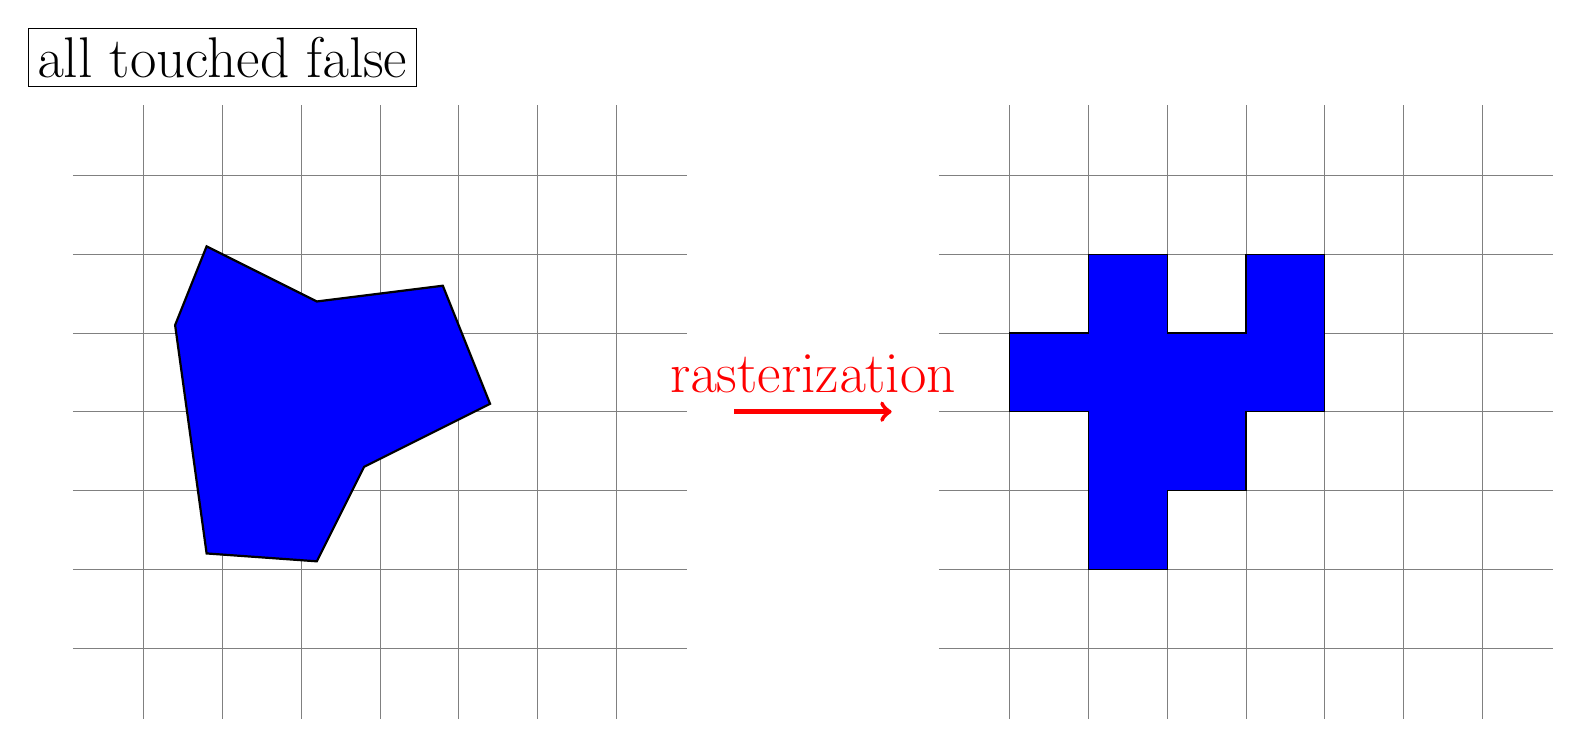
\begin{tikzpicture}
				\node[draw] at (0,6.5) {\huge all touched false};
				\draw[step=1cm,gray,very thin] (-1.9,-1.9) grid (5.9,5.9);
				\draw[fill=blue, thick] (-0.2, 0.2)--(-0.6, 3.1)--(-0.2,4.1)--(1.2,3.4)--(2.8,3.6)--(3.2, 2.6)--(3.4, 2.1)--(1.8,1.3)--(1.2, 0.1)--cycle;
				
				\draw[ultra thick,->, red] (6.5, 2) --node[above=1mm] {\huge rasterization} (8.5, 2);
				
				\draw[step=1cm,gray,very thin] (9.1,-1.9) grid (16.9,5.9);
				\draw[fill=blue] (11,0)--(11,2)--(10,2)--(10,3)--(11,3)--(11,4)--(12,4)--(12,3)--(13,3)--(13,4)--(14,4)--(14,2)--(13,2)--(13,1)--(12,1)--(12,0)--cycle;
			\end{tikzpicture}%
		}%
		\vspace*{5mm}
		\resizebox{8cm}{!}{
			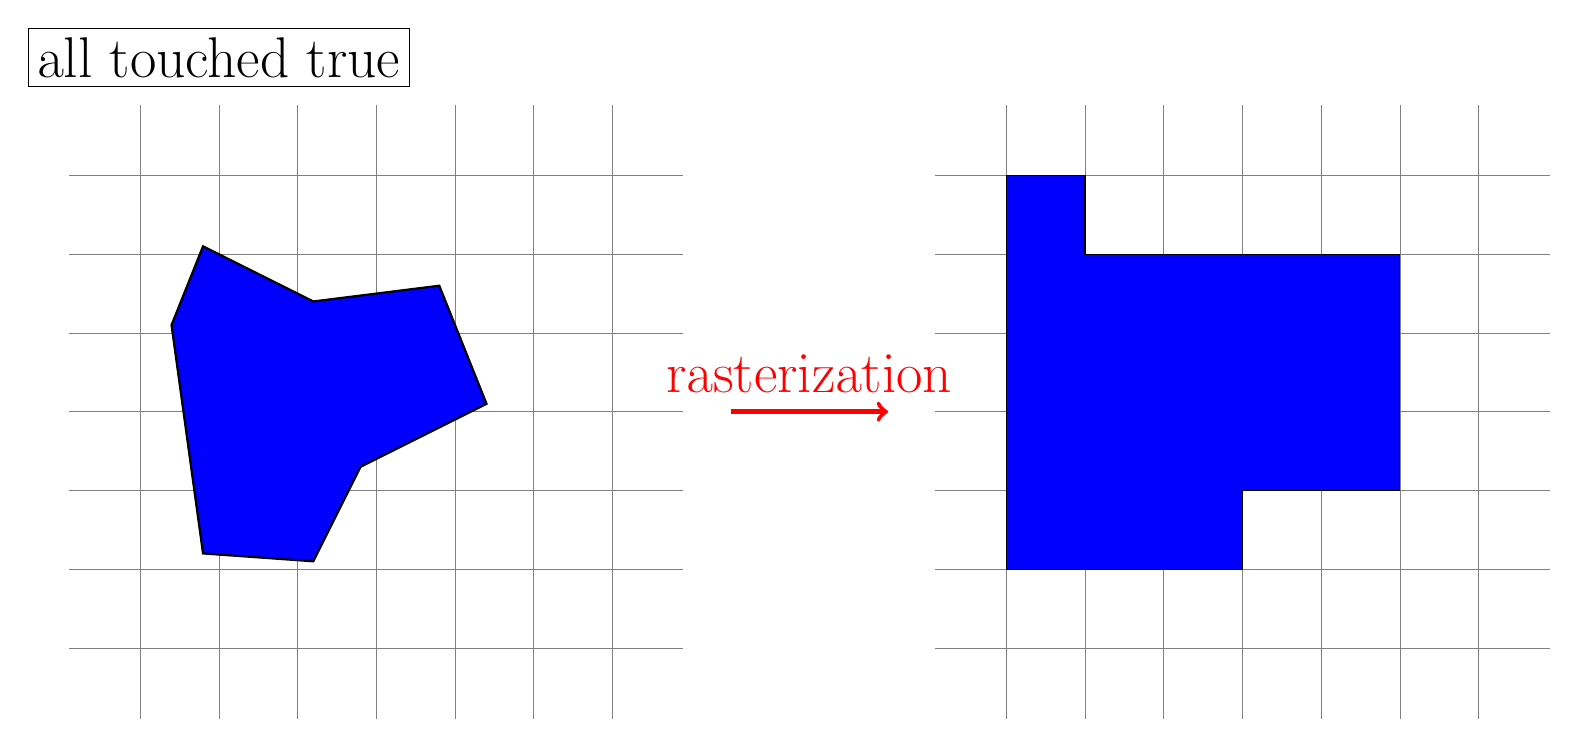
\begin{tikzpicture}
				\node[draw] at (0,6.5) {\huge all touched true};
				\draw[step=1cm,gray,very thin] (-1.9,-1.9) grid (5.9,5.9);
				\draw[fill=blue, thick] (-0.2, 0.2)--(-0.6, 3.1)--(-0.2,4.1)--(1.2,3.4)--(2.8,3.6)--(3.2, 2.6)--(3.4, 2.1)--(1.8,1.3)--(1.2, 0.1)--cycle;
				
				\draw[ultra thick,->, red] (6.5, 2) --node[above=1mm] {\huge rasterization} (8.5, 2);
				
				\draw[step=1cm,gray,very thin] (9.1,-1.9) grid (16.9,5.9);
				\draw[fill=blue] (10,0)--(10,5)--(11,5)--(11,4)--(15,4)--(15,1)--(13,1)--(13,0)--cycle;
			\end{tikzpicture}%
		}%
		\caption{Graphical example for rastering a vector (left blue), to a raster (right blue) with weither all-touched False (above), or all touched True (below).}
		\label{fig:alltouched}

	\end{figure}
	
	\begin{table}[h!]
		\caption{Used levels of costs, the applied numerical equivalent and example layer this cost have been used for.}
		\label{tab:1}
		\centering
		\begin{tabular}{ l  r  l }
			Cost Level 			& Cost 					& Example\\
			\hline
			Prohibited 			& 500					& \makecell[lt]{Conversation areas as\\ National Parks, Buildings} \\
			strongly Restricted & 10 					& \makecell[lt]{Conversation areas as Bird Reserve} \\
			Restricted 			& 5						& \makecell[lt]{Protected Landscape Area,\\ Industrial Areas, motorway, railway} \\
			No Restriction 		& 0.5					& Default\\
			Preferential 		& 0.1					& \makecell[lt]{Power Grid,\\ Motorway and Railway Buffers}\\
		\end{tabular}
	\end{table}
	The completed list of layers and the processing applied to them, can be found in Supplement S1. \todo{create the Supplement from the processing rules}

	\section{Results}\label{sec:results}
	In this chapter we want to show the different cost raster, that were created from the very same set of layers,
	but computed for different resolutions.
	From this different raster the cost paths are calculated and compared.
	In the last step the raster with lower resolution were used to calculate in a way, that they shall result in
	similar paths as if the paths were computed from a high resolution raster.
	\subsection{Cost Raster}\label{subsec:cost-raster}

	The cost raster contains all the costs as weights for the geographic region of the study area.
	The regions outside the study area are given, a no-data value and will not be use for the calculation of the least cost path.
	It is decided to use the maximum value, for any place in the raster, that is covered by several rules at the same time.
	When the resolution that is use for the rasterization is smaller than the object size, than the effect of the rasterization with all touched True or False is limited.
	For all touched True any part of the pixel that is covered by the object, will attribute that whole pixel to the object.
	Thus, the object appears to be halve a pixel size larger in all directs.
	As can be seen in figure~\ref{fig:costs_5m} that shows a detailed view of the costs for village of Beverstedt.
	Due to the maximum aggregation of the costs, the average cost of the raster of all touched true will be over estimated.
	All touched false will be a better description of the real size of the object.
	\begin{figure}
		\centering
		
		\subfloat[\centering All touched: True.]{{\includegraphics[width=.45\linewidth]{./images/CostRaster_5m_alT.png} }}%
		\qquad
		\subfloat[\centering All touched: False.]{{\includegraphics[width=.45\linewidth]{./images/CostRaster_5m_alF.png} }}%
		\caption{Figures of the cost raster. Contrasting the for different values in all touched at a resolution of 5~m.}
		\label{fig:costs_5m}
	\end{figure}
	
	In contrast when the resolution the is much less, than the size of the object the described behavior changes.
	On one hand, while the area, of the pixel is increased for all touched True, also the area for which the cost is overestimated increases.
	On the other hand while the pixel size for all touched  False increases, not only the over estimated area increases for that pixel as describes for all touched true, but in addition the object is less probable situated in the center of the pixel.
	The consequence of the pixel is, that will decreasing resolution that object is not included in the rasterziation.
	Hence, hence for all touched false lower resolution  leads ot a loss of information.
	Because the default is relative small compared the over effect is a underestimation of the costs.
	The figure~\ref{fig:costs_100m} shows for the resolution of 100 m, that while larger are still included in the map they appear to be much larger.
	On the contrary smaller objects might not be included.
	Objects that are small on in one dimension as streets will be included in a stochastic manner.
	Described by the likely of that a object of that sized overlaps with the pixel center.
	\begin{figure}
		\centering
		
		\subfloat[\centering All touched: True.]{{\includegraphics[width=.45\linewidth]{./images/CostRaster_100m_alT.png} }}%
		\qquad
		\subfloat[\centering All touched: False.]{{\includegraphics[width=.45\linewidth]{./images/CostRaster_100m_alF.png} }}%
		\caption{Figures of the cost raster. Contrasting the for different values in all touched at a resolution of 100~m.}
		\label{fig:costs_100m}
	\end{figure}
	Thus, with having larger areas and more objects, with higher costs, all touched True rasterization might more likely lead to longer roots and more likely in blocking the  direct spatial path.
	
	\subsection{Least Cost Paths}\label{subsec:least-cost-paths}
	For each resolution the costs paths were estimated for the rasterization with setting all\_touched False
	and all\_touched True.
	The distance of both paths is calculated with the mean minimum distance.
	For every vertex $P_i$ in the path $L_1$ the minimum between the vertex and the path $L_2$
	is computed and afterwards the minimum distances are averaged (see equation~\ref{eq:1}).
	\begin{equation}
		\label{eq:1}
		d_{mean} = \frac{1}{|L_1|} \sum_{i=1}^{n} d_{min}(p_i, L_2) \bigg\vert p_i \in L_1
	\end{equation}

	Hence, the mean minimum euclidean distance between the two paths can used to compute
	the similarity.
	As different table~\ref{tab:2} shows the distance between the two paths decreases
	with increasing resolution.
	In addition, this tendency is depicted in figure~\ref{fig:paths_resolution} for the calculated cost paths of 5m and 100 m resolutions.
	
	At the same time the differences in the aggregated costs stay constant.
	\todo{Interpretation} When normalize the aggregated costs by the resolution.
	Than On one hand it can be seen, that the all\_touched False under estimate the costs and that this tendency scales
	linear with the resolution.
	On the other hand, the all\_touched True least cost over estimates the aggregated costs on a linear scale of
	the resolution.
	Therefore, the difference for the normalized least cost paths is reduced on scale by the resolution.\todo{show map}
	
	\begin{figure}
		\centering
		
		\subfloat[\centering resolution of 5 m.]{{\includegraphics[width=.45\linewidth]{./images/LeastCostPaths_5m.pdf} }}%
		\qquad
		\subfloat[\centering resolution of 100 m.]{{\includegraphics[width=.45\linewidth]{./images/LeastCostPaths_100m.pdf} }}%
		\caption{Figures of the least cost paths. Contrasting the paths for different resolutions. Paths computed from all touched false raster are indicated by dashed lines. Results from all touched True are indicuated by continuous lines. Higher resolutions are indicated by the color green, lower resolutions by the color red. Using OpenStreetMaps as base map.}
		\label{fig:paths_resolution}
	\end{figure}

	\begin{figure}
		\centering
		
		\subfloat[\centering all touched false.]{{\includegraphics[width=.45\linewidth]{./images/LeastCostPaths_al_F.pdf} }}%
		\qquad
		\subfloat[\centering all touched true.]{{\includegraphics[width=.45\linewidth]{./images/LeastCostPaths_al_T.pdf} }}%
	
		\caption{Figures of the least cost paths. Contrasting the changes of the least cost paths for the different results, depending on the parameter all\_touched. Paths computed from all touched false raster are indicated by dashed lines. Results from all touched True are indicuated by continuous lines. Higher resolutions are indicated by the color green, lower resolutions by the color red. Using OpenStreetMaps as base map.}
		\label{fig:paths_alltouched}
	\end{figure}
	
	\begin{table*}[t]
		\caption{Least cost paths as length for the different \acrfull{res} of the rasters, including the \acrfull{mmd} and the \acrfull{agg} costs. From the \acrshort{agg} costs the differences of the \acrshort{agg} costs and the \acrfull{corr} \acrshort{agg} by resolution are given.} 
		\label{tab:2}
		\centering
		\begin{tabular}{ r  r  r  r  r  r  r  r  r}
			\acrshort{res} /m & $length_{\acrshort{al}=\acrshort{f}} /m$ & $length_{\acrshort{al}=\acrshort{t}} /m$ & \acrshort{mmd} /m & \acrshort{agg}  $ cost_{\acrshort{al}=\acrshort{f}}$ & \acrshort{agg}  $ cost_{\acrshort{al}=\acrshort{t}}$ &  $\Delta $ costs & \acrshort{corr} \acrshort{agg} $costs_{\acrshort{al}=\acrshort{f}}$ & \acrshort{corr} \acrshort{agg} $costs_{\acrshort{al}=\acrshort{t}} $ \\
			\hline
			5 	& 76136.27	& 78002.00 &  126.04 & 18665.923 & 19616.756 & -850.00 & 93329.60 &  97584.77 \\
			10 	& 75430.10 	& 77936.57 &  277.92 &  8931.245 &  9731.175 & -799.95 & 89312.45 &  97311.75 \\
			50 	& 76135.02	& 70619,95 & 1140.01 &  1409.023 &  2300.073 & -891.05 & 70451.15 & 115003.65 \\
			100 & 76283.80	& 74120.73 & 1946.41 &   640.516 &  1572.268 & -931.70 & 64051.60 & 167226.80 \\
	
		\end{tabular}
	\end{table*}
	
	Comparing the all\_touched True rasterization and all\_touched False for the same resolution in contrast with the paths of all\_touched False rasterization at the
	different resolutions the later paths are more similar.
	The mean average distance between the 100 m resolution run and the 5 m resolution run is 257.97 m. \todo{Option add 2.5 m and 25 m}
	
	The similarity of all all\_touched False runs is higher than, the similar between the all\_touched False and all\_touched True runs with the same resolution, except for the highest resolution.
	
	Hence, in an overall perspective paths of the all\_touched False runs stay in a
	similar region, while paths of the all\_touched True coverage strongly to the paths all\_touched False runs.
	This behaviour is depicted in figure~\ref{fig:paths_alltouched}.
	On a more detailed level, it can be seen, that also the Paths of all\_touched 	converges the all\_touched True path.
	But the extent is smaller.
	The length of the the paths only differs to a maximum of about 10 \%.
	The least path distance for higher resolutions can be lower, because new paths, between regions that are forbidden
	in higher resolution can open.
	On the other side the length of the paths can increase, because with higher resolution more vertices will be used.
	
	The zonal stat (see table~\ref{tab:3}) for a buffer of 100 m (5 m) around the path has been used, to estimate the
	percentage of which costs levels are around the path.
	When using all\_touched True rasterization with higher resolution the tendency is to use a higher percentage of the
	Preferential Level and less the NoRestriction Level.\todo{Interpretation:}
	The ratio of the 100 m buffered least cost path, strongly shifted  to Levels lower costs.
	\todo{Interpretation: Interpretation the Cost Paths are much nearer smaller, than 100 m! No problem because buffering is included in the cost raster.}
	There is no strong tendency for the all\_touched False least cost paths.
	
	
	\todo{used regions}
	
	
	\setlength{\tabcolsep}{10pt}
	
	\begin{table*}[t]
		\caption{\acrfull{r} of Category percentages of each least cost path for a buff of 100 m (5 m) around the least cost path.}
		\label{tab:3}
		\centering
		\begin{tabular}{ r  r  r r  r r  r r  r r  r r}
			resolution /m & all touched & \multicolumn{2}{c}{ $ r_{Preferential} \% $}  & \multicolumn{2}{c}{ $ r_{No Restriction} \% $ }  & \multicolumn{2}{c}{ $ r_{Restricted} \% $}  & \multicolumn{2}{ c }{ $ r_{strongly Restricted}\% $ } & \multicolumn{2}{c}{ $ r_{Prohibited} \% $ } \\
			\hline
			5 & False &  4.7  &  (5.4) & 58.7 & (58.9) & 8.8 & (8.4) & 0.7 & (0.7) & 27.1 & (26.7)  \\
			
			10 & False &  19.6 & (33.5) & 68.5 & (64.5)  & 1.0 & (0.8) & 0.8 & (0.3) & 10.1 & (0.9)\\
			
			
			50 & False &  20.4 & (33.2) & 68.0 & (66.2)  & 0.9 & (0.1) & 0.7 & (0.0) & 10.1 & (0.5)\\

			100 & False &  21.1 & (30.7) & 69.1 & (68.8)  & 1.1 & (0.0) & 0.7 & (0.0) & 7.9 & (0.4) \\
			
			\hline
			
			5 & True  &  18.9 & (28.5) & 67.3 & (66.4) & 1.3 & (1.6) & 1.0 & (0.5) & 11.5 & (3.0) \\	
			10 & True &  18.9 & (33.7) & 66.6 & (63.4)  & 1.6 & (1.4) & 1.4 & (0.6) & 11.5 & (1.0)\\	
			50 & True &  9.1 & (13.0) & 75.7 & (83.0) & 3.9 & (2.0) & 4.2 & (1.6) & 7.1 & (0.4) \\
			100 & True &  7.0 & (10.1) & 73.8 & (81.9)  & 5.5 & (3.9) & 8.5 & (3.6) & 5.2 & (0.4) \\	

		\end{tabular}
	\end{table*}

	\todo{Check why values are so different for 5 m all touched False --> simplified line.}

	\subsection{Faster Processing of the Cost Path Algorithm}\label{subsec:faster-processing-of-the-cost-path-algorithm}

	The final least costs paths should between the least cost paths of the lower resolution, with a tendency to be nearer to the paths resulted by the all touched false rasterization.
	The first step is to optimize the calculation speed is, only to calculated the least cost paths for this smaller area.
	Another method, is to improve the prediction of the medium resolution itself and thus reduce the need for a computation in higher resolution.
	\subsubsection{Compare least cost paths, for overlay of both rasterizations}
	As all touched true rasterization overestimates and all touched true underestimates the real costs.
	A weighted mean will describe the real costs more precise.
	As present work indicates, that the weight should favor the all touched false raster.
	The best weight should be the percentage of the pixel, which is covered by the object, but this can not be computed in this work.
	Thus, the best weight has to be searched.
	An alternative might be to compute the cost raster in higher resolution, but than to reproject the to a smaller resolution with a using a (linear) interpolation of the of the weights.\todo{test this idea}
	% \subsubsection{Restrict search to a minimum sized bounding box}
	\subsubsection{Restrict search to a convex hull}
	\todo{Construct a polygon form the two lines. Buffer the polygon.}
	\subsubsection{Restrict search to reachable points}
	For this purpose the aggregated cost as to converted back into a raster.

	\subsubsection{Compare the different Solutions}
	\subsubsection{Check solution for least cost path between different points}
	
	\section{Discussion}\label{sec:discussion}
	As shown need of computation power increases with the power of two with the resolution.
	While the error only scales linear with the resolution.
	
	As the original least cost path QGIS plug-in the used algorithm stops the least aggregation of the costs after the final end point has been found.
	This early stopping might result in sub optimal paths around the end points.
	
	As a any buffer around buildings are describes as protected areas, power poles are also included.
	In further works, these should be excluded.
	
	\todo{discuss aggregation with max vs sum}
	\todo{Scaling with multiple endpoints.}
	\todo{discuss other methods. Off algorithmic speed-ups}
	\todo{discuss other technical methods of speed-ups, as precompilation, JIT, vector units, multi-core}
	\section{Related Works}\label{sec:related-works}


	\section{Conclusion}\label{sec:conclusion}



\begin{acks}
	$\ldots$
\end{acks}

%%
%% The next two lines define the bibliography style to be used, and
%% the bibliography file.
\bibliographystyle{ACM-Reference-Format}
\bibliography{Web_Processing.bib}


%%
%% If your work has an appendix, this is the place to put it.
\appendix

\section{Research Methods}\label{sec:research-methods}

	\subsection{Part One}\label{subsec:part-one}

	\subsection{Part Two}\label{subsec:part-two}


	\section{Online Resources}\label{sec:online-resources}


\end{document}
\endinput
%%
%% End of file `sample-acmsmall.tex'.